
%%%%%%%%%%%%%%%%%%%%%%%%%%%%%%%%%%%%%%%%%%%%%%%%%%%%%%%%%%%%%%
%%     第8章:結論
%%%%%%%%%%%%%%%%%%%%%%%%%%%%%%%%%%%%%%%%%%%%%%%%%%%%%%%%%%%%%%
\chapter{結論}
\label{lbl_chptr5_rslt}

本論文では,マルチメディアデータ処理を効率的に行う
CAMベースマルチメディアデータ処理LSIアーキテクチャの研究を行った.
従来のマルチメディアデータ処理LSIでは,処理全体の30\%から40\%を占めるためボトルネックとなっていた
テーブルルックアップ処理を符号化テーブル最適化ブロックを有するCAM,及びマルチポートCAMを用いることにより,高速かつ,高圧縮に実現
できるアーキテクチャを提案した.
また繰り返し演算処理に対しては,2,048並列の演算器で処理できるCAMを有する超並列SIMD型アーキテクチャを提案した.
この2つのアーキテクチャを融合させることで,マルチメディアアプリケーションの処理効率を
全体的に向上させることが可能となり,その有効性を示すことができた.

本論文で得られた研究成果を,各章ごとにまとめて,
\ref{lbl_chptr5_seika}節に示す.
その後,\ref{lbl_chptr5_ftr}節で本研究に関する今後の応用や将来展望を示す.

%==========================================
% 研究成果
%==========================================
\section{研究成果}
\label{lbl_chptr5_seika}
%--------------------------------------------------------------------------
%		第2章:CAMベースリアルタイム符号化
%--------------------------------------------------------------------------

第\ref{lbl_chptr3}章では,マルチメディアアプリケーションにおける代表的な
テーブルルックアップ処理であるハフマン符号化について,
符号化テーブルの切り替えを行い従来の方式よりも高圧縮にデータを処理することのできるアーキテクチャを提案,
その性能を評価した.

従来の研究は静的ハフマン符号化適用時において,データの圧縮率を
考慮しないものが多かった.
また,考慮した場合においても,あらかじめ複数枚のテーブルを用意する手法を採用し,ハードウェア量の
増加が問題となっていた.
本章の研究は,静的ハフマン符号化における高圧縮処理を2つのテーブルを用意することで
どのようなデータに対しても柔軟に対応できるようにした,実用性に富むものである.

\begin{description}
\item[(2-1)] \underline{ハフマン符号化処理と並列に,符号化テーブルをマルチメディアデータの} \\
\underline{出現頻度にあわせてカスタマイズし,データの圧縮率を向上させることの} \\
\underline{できるアーキテクチャを開発した.}\\
提案アーキテクチャは,CAMを用いて高速にハフマン符号化を行いながら,
データの出現頻度をカウンタによって算出する.
この算出結果を元に,出現頻度の高いデータは別に用意しているカスタマイズ用の符号化テーブル
に最適な符号が割り当てられる.この処理を符号化と並行して行い,
適時切り替えることによってデータの圧縮率を向上させることが可能となる.

\item[(2-2)] \underline{提案アーキテクチャをFPGAに実装しSoC実装が可能であることを示した.} \\
提案アーキテクチャをFPGAに実装し,エンコーダ (符号化モジュール)とオプティマイザ (テーブル更新/切り替えモジュール)の
面積比を確認した.従来のアーキテクチャはエンコーダのみの場合が多いが,提案アーキテクチャの
全体の面積は,エンコーダの約1.9倍であることが分かった.
これをもとに,90 nm 7Cu CMOSテクノロジでのフルカスタム実装面積を見積もった結果,約0.35 mm$^2$
であり,一般にモバイル機器向けSoCコアの面積は1 cm$^2$程度であるため,十分実装可能であることを示した.

\item[(2-3)] \underline{JPEGアプリケーションに適用し,画像の圧縮率向上の有効性を示した.} \\
%JPEGにおけるハフマン符号化をターゲットアプリケーションとし,
解像度が,598 $\times$ 512から,1,500 $\times$ 1,125のベンチマーク画像を用意し,
従来の静的ハフマン符号化アーキテクチャと提案アーキテクチャによる,リアルタイム符号化テーブル
最適化処理の圧縮サイズを比較した.
JPEGにおけるハフマン符号化をターゲットアプリケーションとし,圧縮サイズを算出した結果,
最大28\%の画像サイズ圧縮効果を確認できた.
この差異は,画像の解像度が大きくなるにつれてより明確に効果があるものといえる.
また,今回用いたベンチマーク画像を4 Gbyteのフラッシュメモリに格納する場合,提案アーキテクチャによって
圧縮した画像は240 Mbyte多く格納できることになり,その有効性を示した.

\item[(2-4)] \underline{JPEGアプリケーションに適用時の処理速度向上を実現した.} \\
上記の(2-3)と同一の条件で,ハフマン符号化時の処理速度を算出した結果
デジタルカメラや携帯電話等で,求められている速度仕様である2,3 fpsを十分に
満たしており,将来的に要求されると考えられる5 fps以上も満たしていることが分かった.

\end{description}


第\ref{lbl_chptr4}章では,マルチメディアアプリケーションにおいて
高速処理のボトルネックとなっている,テーブルルックアップ処理を
並列化によって高速化するアーキテクチャを提案,その有効性を示した.

本章の研究によって,従来実現することが難しかったマルチポートCAMを,
他の研究に先駆けて開発することに成功した.
また開発のみにとどまらず,実アプリケーションに適用することでマルチポートCAMの
効果を示すことができた.

\begin{description}
\item[(3-1)] \underline{CAMに複数の入出力ポートを実装したマルチポートCAMを提案した.} \\
単一のメモリセルアレイを複数のポートで共有し,柔軟に効率的な並列一致検索処理が実現できる,
FMCAM (Flexible Multi-ported Content Addressable Memory)を提案した.
従来,並列一致検索処理を実現する場合,CAM等の検索モジュールを複数の用意する必要があったが,
ハードウェア量の増加が著しく,モジュール間のデータコヒーレンシをとるのが難しいため実現は困難であった.
FMCAMはビットパラレル・ブロックパラレル方式,格納データのカテゴリ分け,及び検索時の
ループカウンタの採用でマルチポート化に伴う比較器の増加を最小限にし,
柔軟かつ効率的な並列検索処理を実現した.
また,比較器とメモリセルを分離することで,CAMの特徴を持ちながら,通常の
カスタマイズされたSRAMセルの使用を可能とし,小面積化,低消費電力化
が可能であることを示した.

\item[(3-2)] \underline{FMCAMをFPGAに実装し処理性能の高さを示した.} \\
FMCAMをFPGAに実装し,処理速度,及び面積の両面から総合的な性能を評価した.
評価対象のCAMはソフトマクロ,及びハードマクロから様々な仕様のものを選択し,
評価指標はAT (Area Time)積を使用した.
検証の結果,ビット幅128,ワード数1,024のFMCAMが,他のCAMと比べて約60\%以上小さい値
となり,高性能であることを示した.


\item[(3-3)] \underline{FMCAMのポート数に伴うハードウェア増加率は小さいためスケーラ }\\
\underline{ビリティがあることを示した.} \\
FMCAMは,比較器とメモリセルアレイを分離していることで,ポート数の増加に関わらず
ハードウェア量の増加が抑えられている.
カテゴリ分けを施していない単純なマルチポートCAMと通常のシングルポートCAM
を並列に配置した並列CAMを用意し,ポート数増加に伴うハードウエア量の増加を
FMCAMと比較したところ,ポート数4の場合,並列CAMはFMCAMの約2.36倍ハードウェア量が増加する.
そのため提案FMCAMは面積効率が高いことを示せた.

\item[(3-4)] \underline{テーブルルックアップ処理向けにFMCAMのアーキテクチャを開発した.} \\
FMCAMをテーブルルックアップ処理に適用するために,比較クロックサイクル数の削減を実現する
工夫を施したAdapted FMCAMを提案した.
テーブルルックアップ処理は,符号化前のデータと符号化後のデータが1対1であることに着目し,
一致検索結果が出力された後,直ちに次の検索動作を実行できるシングルサーチモードを導入した.
また,適用アプリケーションによって1カテゴリに格納されるデータ数が異なるため,
ループアドレスカウンタ値を任意に設定できる仕様にした.
これらのアプリケーションオリエンティッドの改良の結果,これまでのFMCAMと比較して約50\%のクロックサイクル数削減を
実現し,その有効性を示した.

\item[(3-5)] \underline{Adapted FMCAMをFPGA/ASICに実装し,スケーラビリティの高さ} \\
\underline{を示した}\\
Adapted FMCAMをFPGAに実装し,次に90 nm 7Cu CMOSテクノロジでのASICの論理合成を行った.
ポート数を1から16まで変化させて動作周波数を確認したところ,
FPGA,及びASIC共に,ハードウェア量は線形に増加することが分かった.
通常のマルチポートメモリは,ポートの増加に伴い面積が2乗に比例した形で増加する.
しかしながら,Adapted FMCAMは,ポートの増加時に追加されるのは
ポートモジュールのみであるため,面積の増加が抑えられているといえる.
また,ポート数の増加に関わらず動作周波数の減少が少ないことを示した.
特にASICにおいてはハードウエア量の増加が線形で一定であるにもかかわらず,
制約条件の200 MHzを下回ることは無い.
この結果によって,Adapted FMCAMは,ポートの増加に対し
スケーラブルであり,その拡張性の高さを立証した.

\item[(3-6)] \underline{並列テーブルルックアップ処理をJPEGアプリケーションに適用し,} \\
\underline{その高速処理を実現した.} \\
Adapted FMCAMをJPEGアプリケーションに適用し,ハフマン符号化における
並列符号化処理の効果を検証した.
解像度が,154 $\times$ 144から,1,024 $\times$ 768のベンチマーク画像を用意し,
従来の静的ハフマン符号化アーキテクチャとAdapted FMCAMによる,ハフマン符号化に
必要なクロックサイクル数を算出した.
その結果,従来のFMCAMに対しクロックサイクル数を約43\%削減し,DSPとの比較では
約93\%の削減を実現した.
これにより並列テーブルルックアップ処理の効果の高さを示した.

\item[(3-7)] \underline{Adapted FMCAMの小面積実装と単位面積当たりの高性能を示した.} \\
(3-6)において,Adapted FMCAMの並列テーブルルックアップ効果を示したが,
実装時の面積も考慮することで,更に検証を行った.
ポート数の増加に伴う単位面積当たりの処理能力を評価に用い,
従来のFMCAMと複数個のDSPを並列に配置した並列DSPとで比較した.
比較の結果,ポート数16の場合において従来のFMCAMの約1.7倍,DSPの約3.8倍
単位面積当たりの処理能力が高いことを示した.
また,Adapted FMCAMは,ポート数を増加するほどこの値は向上するため,
マルチメディアデータ処理LSIに並列テーブルルックアップ処理用のコアとして
組み込むことの有効性を示した.

\item[(3-8)] \underline{Adapted FMCAMとリアルタイムテーブル符号化アーキテクチャとの融合 } \\
\underline{アーキテクチャを提案した.}\\
Adapted FMCAMの並列テーブルルックアップアーキテクチャに,第\ref{lbl_chptr3}章
で有効性を示したリアルタイムテーブル符号化アーキテクチャを融合した,
テーブルルックアップを高速かつ高圧縮に処理できるアーキテクチャを提案した.
提案アーキテクチャは,FMCAMとマルチポートメモリを組み合わせて,並列な
テーブルルックアップ処理を行い,同時にマルチポート向けに改良を加えたオプティマイザに
よって高圧縮処理を行うことが可能である.

\item[(3-9)] \underline{Adapted FMCAMとリアルタイムテーブル符号化の融合アーキテクチャ} \\
\underline{によるJPEGアプリケーションの高速処理を実現した. } \\
(3-8)で提案したアーキテクチャを用いて,
解像度が,192 $\times$ 128から,1,024 $\times$ 768のベンチマーク画像に対して
処理速度と圧縮サイズの算出を行った.
その結果,従来のDSP,もしくはSRAMベース及びCAMベースのエンコーダと比較して
約3倍から20倍の処理速度の向上を確認した.
また画像の圧縮サイズに関しては,平均20\%の圧縮率向上を確認できた.

\end{description}

第\ref{lbl_chptr5}章では,マルチメディアアプリケーションにおいて
テーブルルックアップ処理と並んで,もう1つの処理である,繰り返し演算処理の
高速化を実現するアーキテクチャを提案した.
そして,提案アーキテクチャを第\ref{lbl_chptr3}章及び第\ref{lbl_chptr4}章
で示したCAMベースのテーブルルックアップアーキテクチャと融合することで
マルチメディアアプリケーションを高効率に処理することのできる
アーキテクチャを実現した.

本章の研究によって,性質が異なる上記2つの処理を,
並行して効率よく処理できる
マルチメディアデータ処理LSIの開発を実現することができた.
効率よい両立化の実現は,従来のマルチメディアアプリケーション処理のボトルネックを
解消した新規性の高いものである.

\begin{description}
\item[(4-1)] \underline{超並列SIMD型演算アーキテクチャを提案した.} \\
従来のDSPや専用ハードウェアは,ワードシリアルにデータの処理を行っていたが,
データの処理ベクトルを変更することで,ビットシリアルにデータを処理する
超並列SIMD型演算アーキテクチャを提案した.
提案アーキテクチャは,メモリレジスタ部と演算器を混載することにより
広いバンド幅と低消費電力化を実現し,1,024から2,048という高い並列度を
実現した.

\item[(4-2)] \underline{超並列SIMD型演算アーキテクチャをASICへ実装し,高い処理性能 }\\
\underline{を示した.} \\
超並列SIMD型演算アーキテクチャを共同研究で開発した.
90 nm 7Cu CMOSテクノロジを用いて開発した結果,
面積が3.1 mm$^2$,消費電力が250 mW@200 MHzであり,
処理能力を従来のDSPと比較した.
その結果16 bit加算時において,
単位面積当たりの処理能力が約70倍,
消費電力当たりの処理能力が約12倍と,
共に高い値を示すことでき,マルチメディアデータ処理LSIの繰り返し演算を行うコアとして
有効であることを示した.

\item[(4-3)] \underline{超並列SIMD型演算アーキテクチャとCAMベースのテーブルルックアップ}\\
\underline{アーキテクチャの融合を実現した.} \\
超並列SIMD型演算アーキテクチャの直交インターフェース部に
CAMを組み込むことにより,マルチメディアアプリケーションを構成するテーブルルックアップ処理と
繰り返し演算処理を,どちらも高効率に処理することのできる,
アーキテクチャであるCAMベース超並列SIMD型演算アーキテクチャを提案した.
融合に際しては,SRAM,CAM,直交SRAM,及び直交CAMのうち要求性能を
満たす組み合わせを検討し,直交SRAMが2つ,2バンクのCAMが1つの構成が最適であることが分かった.
また,これらの回路をプログラマブルに動作させるため,
アドレス空間,命令セットやコントローラの仕様を決定し,プログラマブルなアーキテクチャを実現した.

\item[(4-4)] \underline{CAMベース超並列SIMD型演算アーキテクチャをFPGA/ASICに実装し}\\
\underline{高い処理性能を示した.} \\
提案アーキテクチャをFPGAに実装し,USBインターフェースを用いて
PCからのコンソールアプリケーションより基本動作の確認を行った.
次に,\\90 nm 7Cu CMOSテクノロジを用いて論理合成を行った.
直交SRAMセルアレイをフルカスタムで作成し,CAM,直交SRAM,及びコントローラの
面積及び消費電力の見積もりを算出した結果,約0.39 mm$^2$,約32.4 mW@200 MHz
と高性能を実現した.この結果と,(4-2)で示した結果を考慮した場合,全体の面積は約3.49mm$^2$,
消費電力は,200 mW@200 MHzとなり,
一般にモバイル機器向けSoCコアの面積は約1 cm$^2$程度であるため,実装には十分小さい面積で
実現可能であることを示した.

\item[(4-5)] \underline{CAMベース超並列SIMD型演算アーキテクチャによるJPEGアプリケー }\\
\underline{ションの高速処理を実現した}\\
提案アーキテクチャを用いて,JPEGアプリケーションにおけるDCTや量子化等の繰り返し演算処理を,超並列SIMD型演算アーキテクチャで,
ハフマン符号化をCAMによるテーブルルックアップ符号化によって処理した.
解像度が,192 $\times$ 128から,1,500 $\times$ 1,125の
ベンチマーク画像に対してJPEG全体の処理クロックサイクル数を算出した結果,
従来のDSPと比較して,約87\%のクロックサイクル数削減を実現した.
また,単位面積当たりの処理能力は200 MHzでDSPの約4.4倍となり,
CAMベース超並列SIMD型演算アーキテクチャはマルチメディアデータ処理LSI向けの
SoCコアとして大変有効であることを立証した.

\end{description}

%==========================================
% 研究成果の応用と将来展望
%==========================================
\section{研究成果の応用と将来展望}
\label{lbl_chptr5_ftr}

本研究では,大量のマルチメディアデータを高速,高圧縮に処理することのできる
CAMベースの高性能マルチメディアデータ処理LSIアーキテクチャを開発した.
以下に,今後の研究成果の応用と将来展望について示す.

%
%==========================================
% 研究成果の応用
%==========================================
\subsection{研究成果の応用}

本研究成果の今後の応用として,主として以下の3つが挙げられる.
\begin{list}{}{}
\item[(1)] 暗号や誤り訂正処理等のアプリケーションに対する効率的な圧縮処理.
\item[(2)] ルーティング処理やマルチコアキャッシュへの並列一致検索処理の応用.
\item[(3)] CAMベース超並列SIMD型演算アーキテクチャのモバイル機器用アプリケーションへの応用
\end{list}{}{}

\begin{itemize}
\item[(1)]近年携帯電話をはじめとするモバイル機器,家庭用ゲーム機,及びデジタル家電等
は多機能化が進んでいる.そのためこれらの機器に搭載されるLSIは,音声,動画像の処理を始め,
安全な通信のための暗号や誤り訂正処理等のアルゴリズムを効率よく処理できる能力が求められる.
特にモバイル機器においては,取り扱うデータ量の増大に対し効率よく圧縮処理を行い
転送データ量を抑える工夫が必要となる.
しかしながら,暗号や誤り訂正処理においては従来の動画像に用いられている不可逆な圧縮 (復号時にデータの欠損
が生じる)方式は適用できない.
従って,可逆圧縮方式をうまく用いて高圧縮を実現する必要がある.
本研究で提案したCAMベースのリアルタイム符号化テーブル最適化アーキテクチャは,
ハフマン符号化を圧縮アルゴリズムに用いているため可逆圧縮であり,CAMを用いているため
リアルタイムに符号化を実現しながら,圧縮効率の向上も実現できる.
このアーキテクチャを先に述べたLSIのコアとして応用することで,
様々はアプリケーションに対して今後増大するデータ量の圧縮を効率よく実現することが期待される.

\item[(2)]現在,並列一致検索処理が有効であると考えられる応用例として
ルーティング,マルチコアに対するキャッシュ等がある.
ルーティングに関しては,事業所やプロバイダにおける基幹ルータへの応用が挙げられる.
近年,FTTH等の普及により,基幹ルータにはより高速なルーティングが求められている.
従来このルーティングにはCAMを複数配置して処理を行うことが多かったが,
ここにFMCAMを応用することで,実装面積,処理能力,消費電力,及びルーティングデテーブルのメインテナンス等
様々な利点が得られると考えられる.実際の応用に関しては,FMCAMをターナリ (3値)化し,TCAMとして実装することが考えられる.
またキャッシュに関しては,CPU等のプロセッサでマルチコア化が急激に進む中,これまでキャッシュに使用されていた
CAMにFMCAMを応用することが考えられる.これによって各CPUのコアによるキャッシュテーブルの共有が
可能となり,更にCAMの能力を用いて目的のデータをすばやく検索することが可能になると考えられる.

\item[(3)]本研究では提案したCAMベース超並列SIMD型演算アーキテクチャをJPEGアプリケーションによって
性能を評価した.今後はより広範囲で性能を評価するために動画像や暗号処理,誤り訂正等の
アプリケーションへの適用を検討する.
具体的なターゲットアプリケーションとしては,携帯電話の動画像配信に利用されているMPEG-4,
携帯電話の地上デジタル放送視聴に利用されているH.264がある.
暗号化に関しては,ISO (International Organization for Standardization)/IEC (International Electrotechnical Commission)
にて国際標準暗号に制定されている,AES (Advanced Encryption Standard)やTriple DES (Data Encryption Standard)等がある.
誤り訂正符号方式に関しては,次世代のアルゴリズムであるLDPC (Low Density Parity Check)符合がある.

\end{itemize}

%==========================================
% 将来展望
%==========================================
\subsection{将来展望}

本研究で提案した高性能CAMベースマルチメディアデータ処理LSIアーキテクチャの
将来展望として,更に処理性能を向上図ったプロセッシングアーキテクチャが考えられる.
近年,CPU等のプロセッサにおいてマルチコア化の研究,開発が盛んになっており,
ユーザが容易に入手できるようになってきた.
IntelのCore Duo等のデュアルコアプロセッサは,ノートパソコンにも使用されており,
次世代ゲーム機のプレイステーション3に使われているCellと呼ばれるプロセッサは,9個のコアを
内蔵している.
また,2006年にサンフランシスコで開催されたIntel Developer Forumでは,
コア数が80個であるメニイコアプロセッサの試作品も発表されており,毎秒1 Tbyte/sの浮動小数点演算を可能としている\cite{dicius06}.
このような背景からも,マルチコア化は高性能化への1手法として大変有効であると考えられる.
そこで,今後の研究の拡張として第\ref{lbl_chptr5}章にて述べた,
超並列SIMD型演算モジュールをマルチコア化して,FMCAMを実装させた
階層並列構造SIMD型プロセッシングアーキテクチャが考えられる.
図 \ref{neo_mtx}にその概念図を示す.
階層並列構造SIMD型プロセッシングアーキテクチャは,SIMD型演算モジュールを
並列もしくはインタリーブ動作させることにより大量のデータを並列に処理することが可能であり,
各コアがテーブルルックアップ処理を行う場合にはFMCAMを用いて一致検索処理を行うことが可能となる.
また,圧縮が必要なアプリケーションに対してはオプティマイザを用いることによって
高圧縮な可逆圧縮処理も可能としている.
このアーキテクチャは,並列度を増加することで容易に処理性能を向上させることができるため,
モバイル機器の用途のみならず,デスクトップPCやサーバ向けのコアとしても十分に威力を発揮することが
期待できる.
また,最小距離検索連想メモリを導入することによるあいまい検索処理を用いて,
高度並列知能システムアーキテクチャへ発展することが期待できる


% figure*
	\begin{figure*}[tbh]
	\centering
		\begin{center}
			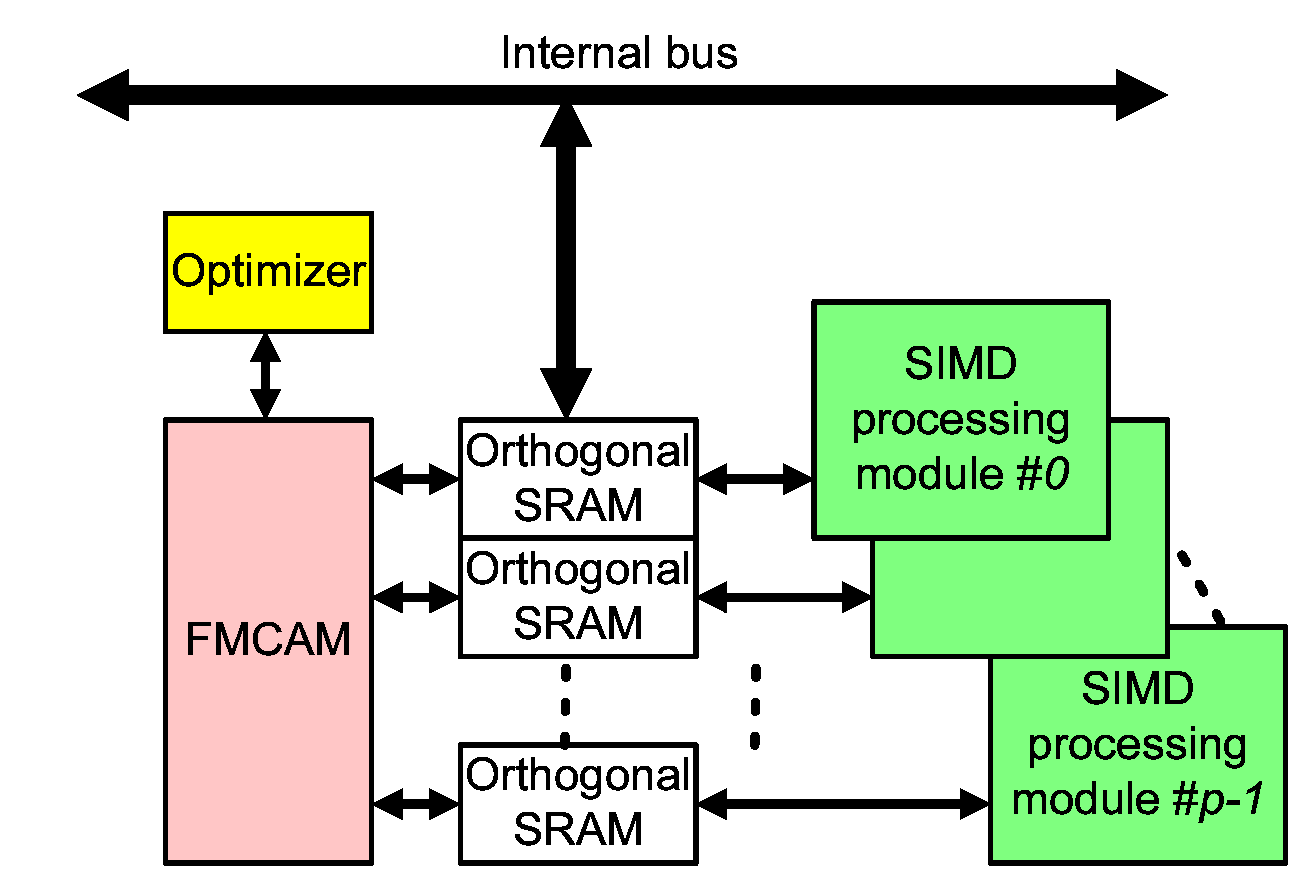
\includegraphics[width = 14cm,  height = 14cm,  keepaspectratio, clip]{./pics/neo_mtx.eps}
		\caption{階層並列構造SIMD型プロセッシングアーキテクチャ.}
		\label{neo_mtx}
		\end{center}
	\end{figure*}%	
%figure*

%-------------------------------------------------------------------- 
\
